\documentclass[12pt,a4paper]{article}

% ---------------------------------------------------------------
% PACKAGES
% ---------------------------------------------------------------
\usepackage{amsmath}
\usepackage{amssymb}
\usepackage{geometry}
\geometry{margin=2.5cm}
\usepackage{booktabs}
\usepackage{xcolor}
\usepackage{hyperref}
\usepackage{listings}
\usepackage{pgfplots}
\pgfplotsset{compat=1.18}
\usepackage{tcolorbox}
\tcbuselibrary{skins, breakable}
\usepackage{enumitem}
\usepackage{fancyhdr}
\usepackage{tikz}
\usepackage{array}

% ---------------------------------------------------------------
% TCOLORBOX ENVIRONMENTS
% ---------------------------------------------------------------
\newtcolorbox{curiositybox}[1]{colback=yellow!10, colframe=orange!80!black, fonttitle=\bfseries, title=#1, breakable}
\newtcolorbox{infobox}[1]{colback=blue!5, colframe=blue!60!black, fonttitle=\bfseries, title=#1, breakable}
\newtcolorbox{mistakebox}[1]{colback=red!5, colframe=red!60!black, fonttitle=\bfseries, title=#1, breakable}
\newtcolorbox{learnbox}[1]{colback=green!5, colframe=green!60!black, fonttitle=\bfseries, title=#1, breakable}

% ---------------------------------------------------------------
% LISTINGS (PYTHON)
% ---------------------------------------------------------------
\lstset{language=Python, basicstyle=\ttfamily\small, keywordstyle=\color{blue},
        commentstyle=\color{gray}, stringstyle=\color{orange},
        showstringspaces=false, numbers=left, numberstyle=\tiny,
        breaklines=true, frame=single}

% ---------------------------------------------------------------
% FANCYHDR
% ---------------------------------------------------------------
\pagestyle{fancy}
\fancyhf{}
\lhead{Topic 06: Unit Step \& Second Shifting}
\rhead{Unit IV --- Laplace Transforms}
\cfoot{\thepage}

% ---------------------------------------------------------------
% TITLE
% ---------------------------------------------------------------
\title{Topic 06: Unit Step Function \& Second Shifting Theorem \\
       \large Unit IV --- Laplace Transforms}
\author{23A54201 --- Mathematics IV (Transform Techniques) \\
        JNTUA College of Engineering (Autonomous)}
\date{}

% ---------------------------------------------------------------
\begin{document}
% ---------------------------------------------------------------
\maketitle
\tableofcontents
\newpage

% ==============================================================
\section{Opening Hook}
% ==============================================================

\begin{curiositybox}{Hook}
Imagine a light switch that stays OFF until exactly $t = 5$ seconds, then suddenly turns ON
and stays on forever.
How do you even write this function mathematically without drawing a picture?
Enter the unit step function --- a mathematical ``switch'' that turns terms on and off at will.
And once you can write delayed functions, the Second Shifting Theorem tells you exactly how
to transform them, no re-derivation needed.
\end{curiositybox}

% ==============================================================
\section{Why This Topic Exists}
% ==============================================================

Before we begin, here is the honest answer to why you are reading this.
Real engineering signals do not cooperate with neat continuous formulas --- they switch on
at a specific moment, pause for a fixed delay, or fire only once and disappear.
A resistor that connects to a voltage source at $t = 2\,\text{s}$, a robotic arm whose
command arrives $0.5\,\text{s}$ after a sensor trigger, a solenoid valve that opens at
$t = 10\,\text{s}$ --- all of these are described naturally using the unit step function.
Without it, every piecewise input requires a separate integral over each sub-interval,
and life becomes complicated very quickly.

The table below shows the typical pitfalls students fall into when they skip this topic and
try to proceed anyway.

\begin{center}
\begin{tabular}{@{}ll@{}}
\toprule
\textbf{What students skip} & \textbf{Consequence} \\
\midrule
Writing piecewise functions the long way
  & Struggling to find their Laplace transform at all \\
Confusing $u(t-a)$ with $u(t) - a$
  & Getting the delay condition completely wrong \\
Forgetting to shift $f(t)$ itself, not just $u(t-a)$
  & Applying the second shifting theorem incorrectly \\
Not recognising the $e^{-as}$ factor in an inverse problem
  & Failing to recover the delayed form from $F(s)$ \\
Mixing the first and second shifting theorems
  & Wrong domain shifted, wrong formula applied \\
\bottomrule
\end{tabular}
\end{center}

\begin{learnbox}{Key Motivation}
The unit step function and the Second Shifting Theorem are the engineer's toolkit for
handling any delayed or switched signal inside the Laplace framework --- cleanly, compactly,
and without breaking into multiple sub-problems.
\end{learnbox}

% ==============================================================
\section{You Already Know This (Intuition First)}
% ==============================================================

Think of a stage performance.
Before the cue the stage light is completely dark --- the stagehand's hand is on the switch
but has not moved yet.
At a pre-scheduled cue time the stagehand flips the switch and the light turns on ---
and it stays on for the rest of the performance.

That is precisely the unit step function $u(t - a)$.
The ``cue time'' is $a$, before which the function outputs zero (dark stage), and at and
after which the function outputs one (light on).
No gradual fade, no partial brightness --- a clean, instantaneous switch.
The beauty is that multiplying any signal $f(t)$ by $u(t-a)$ instantly ``turns on'' that
signal starting at $t = a$, and the Second Shifting Theorem tells you how this multiplication
transforms beautifully into a simple factor of $e^{-as}$ in the $s$-domain.

% ==============================================================
\section{The Unit Step (Heaviside) Function}
% ==============================================================

\begin{infobox}{Definition of the Unit Step Function}
The \textbf{unit step function} (also called the \textbf{Heaviside function}) is defined as:
\[
  u(t - a) \;=\; \begin{cases} 0, & t < a \\ 1, & t \geq a \end{cases}
\]
where $a \geq 0$ is the \emph{delay} or \emph{switch-on time}.
Special case: when $a = 0$,
\[
  u(t) \;=\; \begin{cases} 0, & t < 0 \\ 1, & t \geq 0 \end{cases}
\]
which is the standard unit step at the origin.
The notation $H(t-a)$ is also widely used and is identical to $u(t-a)$.
\end{infobox}

\subsection*{Graph of $u(t-3)$}

The following pgfplots diagram shows $u(t-3)$ over $t \in [0, 6]$, clearly displaying
the jump discontinuity at $t = 3$ using the open/filled circle convention.

\begin{center}
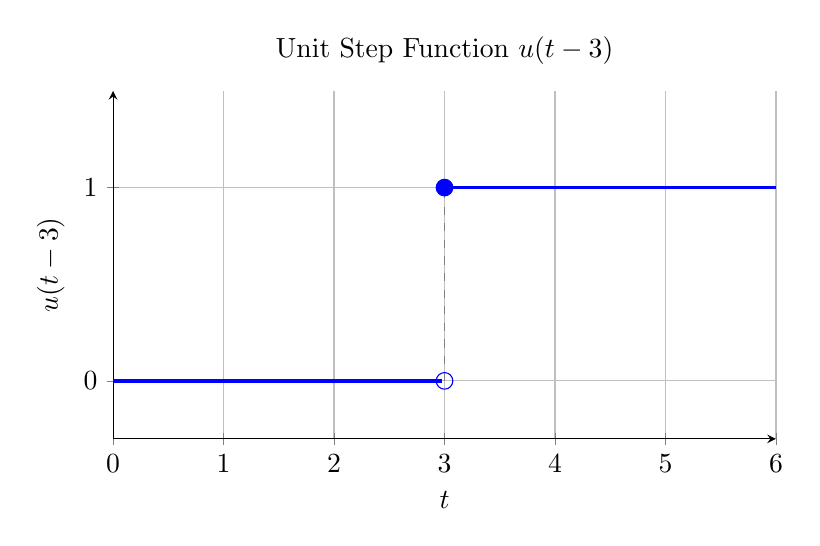
\begin{tikzpicture}
\begin{axis}[
  xlabel={$t$},
  ylabel={$u(t-3)$},
  xmin=0, xmax=6,
  ymin=-0.3, ymax=1.5,
  xtick={0,1,2,3,4,5,6},
  ytick={0,1},
  grid=major,
  width=10cm, height=6cm,
  title={Unit Step Function $u(t-3)$},
  axis lines=left
]
% segment for t < 3: y = 0
\addplot[blue, very thick, domain=0:2.98, samples=2] {0};
% segment for t >= 3: y = 1
\addplot[blue, very thick, domain=3:6, samples=2] {1};
% open circle at (3, 0)
\addplot[blue, only marks, mark=o, mark size=3pt] coordinates {(3, 0)};
% filled circle at (3, 1)
\addplot[blue, only marks, mark=*, mark size=3pt] coordinates {(3, 1)};
% vertical dashed line at t=3
\addplot[dashed, gray, domain=0:1, samples=2] coordinates {(3,0) (3,1)};
\end{axis}
\end{tikzpicture}
\end{center}

The open circle at $(3, 0)$ indicates the function does \emph{not} take the value 0 at
$t = 3$; the filled circle at $(3, 1)$ shows the function jumps to 1 at that exact moment
and remains there.

% ==============================================================
\section{Laplace Transform of the Unit Step Function}
% ==============================================================

\begin{infobox}{Derivation: $\mathcal{L}\{u(t-a)\}$}
Starting from the definition of the Laplace transform:
\[
  \mathcal{L}\{u(t-a)\} \;=\; \int_0^{\infty} e^{-st}\, u(t-a)\, dt
\]
Since $u(t-a) = 0$ for $t < a$ and $u(t-a) = 1$ for $t \geq a$, the integrand is zero on
$[0, a)$, so the lower limit of integration effectively shifts to $a$:
\[
  = \int_a^{\infty} e^{-st} \cdot 1\, dt
  = \left[\frac{e^{-st}}{-s}\right]_a^{\infty}
\]
For $s > 0$ the upper limit gives zero (since $e^{-st} \to 0$ as $t \to \infty$):
\[
  = 0 - \left(\frac{e^{-as}}{-s}\right)
  = \frac{e^{-as}}{s}
\]
\[
  \boxed{\mathcal{L}\{u(t-a)\} = \frac{e^{-as}}{s}, \quad s > 0, \; a \geq 0}
\]
\end{infobox}

\begin{learnbox}{What Did We Learn?}
The Laplace transform of a unit step delayed by $a$ seconds is simply $\dfrac{e^{-as}}{s}$.
The factor $e^{-as}$ encodes the delay; as $a \to 0$ this reduces to $\dfrac{1}{s}$, the
transform of the ordinary step at the origin.
\end{learnbox}

% ==============================================================
\section{Writing Piecewise Functions Using Unit Steps}
% ==============================================================

Any piecewise function can be expressed as a \emph{single formula} by switching different
pieces on and off using unit steps.
The key idea is: to ``turn off'' piece $A$ and ``turn on'' piece $B$ at $t = c$, add the
term $(B - A)\,u(t - c)$.

\textbf{Demonstration.} Express
\[
  f(t) = \begin{cases} t^2, & 0 \leq t < 2 \\ 5, & t \geq 2 \end{cases}
\]
in terms of unit steps.

\textbf{Step 1.} Start with the formula that holds for the first piece: $t^2$.

\textbf{Step 2.} At $t = 2$ we want to switch from $t^2$ to $5$, so we add the
``correction'' $(5 - t^2)\,u(t-2)$:
\[
  f(t) = t^2 + (5 - t^2)\,u(t-2)
\]

\textbf{Verification.}
\begin{itemize}
  \item For $0 \leq t < 2$: $u(t-2) = 0$, so $f(t) = t^2 + 0 = t^2$. \checkmark
  \item For $t \geq 2$: $u(t-2) = 1$, so $f(t) = t^2 + (5 - t^2) \cdot 1 = 5$. \checkmark
\end{itemize}

The representation is exact and holds over the entire domain.

\begin{learnbox}{Technique Summary}
To convert a piecewise function with $n$ pieces into a unit-step expression, start with the
first piece's formula and add one correction term for every boundary where the formula
changes. Each correction term multiplied by the appropriate $u(t - c)$ switches the change
on at $t = c$.
\end{learnbox}

% ==============================================================
\section{Second Shifting Theorem}
% ==============================================================

\begin{infobox}{Second Shifting Theorem (t-Shifting Theorem)}
Let $f(t)$ be a function with Laplace transform $\mathcal{L}\{f(t)\} = F(s)$.
Then the Laplace transform of the \emph{delayed} and \emph{switched} version of $f$ is:
\[
  \boxed{\mathcal{L}\{f(t-a)\,u(t-a)\} = e^{-as}\,F(s)}
\]
Equivalently, in inverse form:
\[
  \mathcal{L}^{-1}\{e^{-as}\,F(s)\} = f(t-a)\,u(t-a)
\]
Both forms hold for $a \geq 0$ and $s$ in the appropriate right half-plane.
\end{infobox}

\begin{learnbox}{Reading the Theorem}
The formula says: delaying a time-domain function by $a$ units (and switching it on at that
moment with $u(t-a)$) is equivalent to multiplying its Laplace transform by $e^{-as}$.
Delay in time $\leftrightarrow$ multiplication by an exponential in $s$.
\end{learnbox}

% ==============================================================
\section{Proof of the Second Shifting Theorem}
% ==============================================================

\begin{infobox}{Proof from First Principles}
\textbf{Goal:} Show $\mathcal{L}\{f(t-a)\,u(t-a)\} = e^{-as}\,F(s)$.

\textbf{Start from the definition:}
\[
  \mathcal{L}\{f(t-a)\,u(t-a)\}
  = \int_0^{\infty} e^{-st}\,f(t-a)\,u(t-a)\,dt
\]
Since $u(t-a) = 0$ for $t < a$ and $u(t-a) = 1$ for $t \geq a$, the lower limit
effectively shifts to $a$:
\[
  = \int_a^{\infty} e^{-st}\,f(t-a)\,dt
\]
\textbf{Substitution:} Let $\tau = t - a$, so $t = \tau + a$ and $dt = d\tau$.
When $t = a$, $\tau = 0$; when $t \to \infty$, $\tau \to \infty$:
\[
  = \int_0^{\infty} e^{-s(\tau + a)}\,f(\tau)\,d\tau
  = \int_0^{\infty} e^{-s\tau}\,e^{-as}\,f(\tau)\,d\tau
  = e^{-as}\int_0^{\infty} e^{-s\tau}\,f(\tau)\,d\tau
\]
The remaining integral is exactly $\mathcal{L}\{f(\tau)\} = F(s)$, giving:
\[
  \mathcal{L}\{f(t-a)\,u(t-a)\} = e^{-as}\,F(s) \qquad \blacksquare
\]
\end{infobox}

% ==============================================================
\section{Contrast: First vs.\ Second Shifting Theorem}
% ==============================================================

Students frequently confuse the two shifting theorems because both involve
an exponential factor.
The table below compares them across five dimensions.

\begin{center}
\begin{tabular}{@{}lll@{}}
\toprule
\textbf{Feature} & \textbf{First Shifting (s-Shifting)} & \textbf{Second Shifting (t-Shifting)} \\
\midrule
What is shifted & $s$-domain (transform variable) & $t$-domain (time variable) \\
\addlinespace
Formula & $\mathcal{L}\{e^{at}f(t)\} = F(s-a)$ & $\mathcal{L}\{f(t-a)u(t-a)\} = e^{-as}F(s)$ \\
\addlinespace
Multiplying factor & $e^{at}$ multiplies $f(t)$ in time & $e^{-as}$ multiplies $F(s)$ in $s$ \\
\addlinespace
Typical use case & Damped sinusoids, decaying exponentials & Switched/delayed inputs, piecewise signals \\
\addlinespace
Example function & $e^{-2t}\sin(3t) \to \dfrac{3}{(s+2)^2+9}$ & $(t-4)^2 u(t-4) \to \dfrac{2\,e^{-4s}}{s^3}$ \\
\addlinespace
Key memory hook & ``$e^{at}$ in time shifts $s$ by $a$'' & ``delay $a$ in time $\Rightarrow\; e^{-as}$ in $s$'' \\
\bottomrule
\end{tabular}
\end{center}

\begin{learnbox}{Quick Distinction}
First shifting: exponential multiplier in \emph{time domain} $\Rightarrow$ shift in $s$-domain.
Second shifting: delay in \emph{time domain} with a unit step $\Rightarrow$ exponential factor in $s$-domain.
\end{learnbox}

% ==============================================================
\section{Worked Examples}
% ==============================================================

% ------------------------------------------
\subsection*{Example 1 --- Direct Application}

\begin{infobox}{Example 1: Find $\mathcal{L}\{(t-2)^2\,u(t-2)\}$}
\textbf{Observe:} The expression $(t-2)^2\,u(t-2)$ is already in the exact form
$f(t-a)\,u(t-a)$ with $a = 2$ and $f(t) = t^2$.

\textbf{Step 1.} Find $F(s) = \mathcal{L}\{f(t)\} = \mathcal{L}\{t^2\}$.
Using the standard formula $\mathcal{L}\{t^n\} = \dfrac{n!}{s^{n+1}}$:
\[
  F(s) = \frac{2!}{s^3} = \frac{2}{s^3}
\]

\textbf{Step 2.} Apply the Second Shifting Theorem with $a = 2$:
\[
  \mathcal{L}\{(t-2)^2\,u(t-2)\} = e^{-2s}\,F(s) = \frac{2\,e^{-2s}}{s^3}
\]

\textbf{Answer:}
\[
  \boxed{\mathcal{L}\{(t-2)^2\,u(t-2)\} = \frac{2\,e^{-2s}}{s^3}}
\]
\end{infobox}

\begin{learnbox}{What Did We Learn? (Example 1)}
When the expression is already in the form $f(t-a)\,u(t-a)$, the Second Shifting Theorem
applies in one direct step: find $F(s)$ and multiply by $e^{-as}$.
Always check first whether the argument of $u$ matches the shift inside $f$.
\end{learnbox}

% ------------------------------------------
\subsection*{Example 2 --- Requires Rewriting}

\begin{infobox}{Example 2: Find $\mathcal{L}\{t^2\,u(t-2)\}$}
\textbf{Warning:} This is \emph{not} in the form $f(t-a)\,u(t-a)$ because the function
multiplying $u(t-2)$ is $t^2$, not $(t-2)^2$.
We must rewrite $t^2$ entirely in terms of $(t-2)$ before applying the theorem.

\textbf{Step 1.} Substitute $t = (t-2) + 2$ and expand:
\[
  t^2 = \bigl[(t-2) + 2\bigr]^2
  = (t-2)^2 + 4(t-2) + 4
\]

\textbf{Step 2.} Therefore:
\[
  t^2\,u(t-2) = \bigl[(t-2)^2 + 4(t-2) + 4\bigr]\,u(t-2)
\]

\textbf{Step 3.} Now each term is in the correct form $g(\tau)\big|_{\tau=t-2}\,u(t-2)$
with $a = 2$.
Apply the Second Shifting Theorem to each piece:
\begin{align*}
  \mathcal{L}\{(t-2)^2\,u(t-2)\} &= e^{-2s}\cdot\frac{2}{s^3} \\[4pt]
  \mathcal{L}\{4(t-2)\,u(t-2)\}  &= 4\,e^{-2s}\cdot\frac{1}{s^2} \\[4pt]
  \mathcal{L}\{4\,u(t-2)\}        &= 4\,e^{-2s}\cdot\frac{1}{s}
\end{align*}

\textbf{Step 4.} Sum the three results:
\[
  \mathcal{L}\{t^2\,u(t-2)\} = e^{-2s}\!\left(\frac{2}{s^3} + \frac{4}{s^2} + \frac{4}{s}\right)
\]

\textbf{Answer:}
\[
  \boxed{\mathcal{L}\{t^2\,u(t-2)\} = e^{-2s}\!\left(\frac{2}{s^3} + \frac{4}{s^2} + \frac{4}{s}\right)}
\]
\end{infobox}

\begin{learnbox}{What Did We Learn? (Example 2)}
When $f(t)\,u(t-a)$ is given but $f(t)$ is \emph{not} in terms of $(t-a)$, always rewrite
$f(t)$ by substituting $t = (t-a) + a$ and expanding before applying the theorem.
Skipping this rewrite is the single most common error on this topic.
\end{learnbox}

% ------------------------------------------
\subsection*{Example 3 --- Inverse Application}

\begin{infobox}{Example 3: Find $\mathcal{L}^{-1}\!\left\{\dfrac{e^{-3s}}{s^2+4}\right\}$}
\textbf{Identify the structure:} The expression has the form $e^{-as}\,F(s)$ with
$a = 3$ and $F(s) = \dfrac{1}{s^2 + 4}$.

\textbf{Step 1.} Find $f(t) = \mathcal{L}^{-1}\{F(s)\}$.
Recall the standard pair $\mathcal{L}\{\sin(bt)\} = \dfrac{b}{s^2+b^2}$, so with $b = 2$:
\[
  \mathcal{L}^{-1}\!\left\{\frac{1}{s^2+4}\right\} = \frac{1}{2}\sin(2t)
\]
Thus $f(t) = \dfrac{1}{2}\sin(2t)$.

\textbf{Step 2.} Apply the inverse Second Shifting Theorem:
\[
  \mathcal{L}^{-1}\{e^{-as}\,F(s)\} = f(t-a)\,u(t-a)
\]
with $a = 3$:
\[
  f(t-3) = \frac{1}{2}\sin\bigl(2(t-3)\bigr)
\]

\textbf{Answer:}
\[
  \boxed{\mathcal{L}^{-1}\!\left\{\frac{e^{-3s}}{s^2+4}\right\}
  = \frac{1}{2}\sin\bigl(2(t-3)\bigr)\,u(t-3)}
\]
The function is zero for $t < 3$ and equals $\dfrac{1}{2}\sin(2(t-3))$ for $t \geq 3$.
\end{infobox}

\begin{learnbox}{What Did We Learn? (Example 3)}
Whenever you see $e^{-as}$ multiplying a standard $F(s)$, the inverse transform is
automatically the corresponding $f(t)$ shifted by $a$, switched on by $u(t-a)$.
Spot the $e^{-as}$, strip it off, invert $F(s)$ normally, then attach the delay.
\end{learnbox}

% ------------------------------------------
\subsection*{Example 4 --- Switched-Circuit ODE}

\begin{infobox}{Example 4: Solve $y' + y = u(t-1)$, $y(0) = 0$}
This models an electrical circuit (RC or RL) where the voltage source is switched on
at $t = 1$ second.

\textbf{Step 1. Transform both sides.}
Taking $\mathcal{L}$ of both sides and using $\mathcal{L}\{y'\} = sY(s) - y(0) = sY(s)$
(since $y(0) = 0$):
\[
  sY(s) + Y(s) = \mathcal{L}\{u(t-1)\} = \frac{e^{-s}}{s}
\]

\textbf{Step 2. Solve for $Y(s)$.}
\[
  Y(s)(s+1) = \frac{e^{-s}}{s}
  \implies
  Y(s) = \frac{e^{-s}}{s(s+1)}
\]

\textbf{Step 3. Partial fractions on $\dfrac{1}{s(s+1)}$.}
\[
  \frac{1}{s(s+1)} = \frac{A}{s} + \frac{B}{s+1}
\]
Multiplying through: $1 = A(s+1) + Bs$.
Setting $s = 0$: $A = 1$.
Setting $s = -1$: $B = -1$.
\[
  \frac{1}{s(s+1)} = \frac{1}{s} - \frac{1}{s+1}
\]

\textbf{Step 4. Identify $F(s)$ and apply inverse Second Shifting Theorem.}
\[
  Y(s) = e^{-s}\!\left(\frac{1}{s} - \frac{1}{s+1}\right) = e^{-s}\,G(s)
\]
where $G(s) = \dfrac{1}{s} - \dfrac{1}{s+1}$.
Inverting $G(s)$:
\[
  g(t) = \mathcal{L}^{-1}\!\left\{\frac{1}{s} - \frac{1}{s+1}\right\} = 1 - e^{-t}
\]
Applying the inverse Second Shifting Theorem with $a = 1$:
\[
  y(t) = g(t-1)\,u(t-1) = \bigl(1 - e^{-(t-1)}\bigr)\,u(t-1)
\]

\textbf{Answer:}
\[
  \boxed{y(t) = \bigl(1 - e^{-(t-1)}\bigr)\,u(t-1)}
\]
This is zero for $t < 1$ and equals $1 - e^{-(t-1)}$ for $t \geq 1$ --- exactly the
step-response of a first-order system delayed by 1 second.
\end{infobox}

\begin{learnbox}{What Did We Learn? (Example 4)}
When the forcing function contains a unit step (a switched source), its transform contains
$e^{-as}$.
After solving for $Y(s)$ and doing partial fractions on the algebraic part, use the inverse
Second Shifting Theorem in the last step to recover $y(t)$ with the correct delay baked in.
\end{learnbox}

% ==============================================================
\section{Excel Example}
% ==============================================================

We numerically verify Example 1: the function $(t-2)^2\,u(t-2)$.

\textbf{Setup.} Column A holds the time values $t = 0, 0.5, 1, \ldots, 6$.
The table below shows the first seven rows of the spreadsheet.

\begin{center}
\begin{tabular}{@{}ccccc@{}}
\toprule
\textbf{Row} & \textbf{A: t} & \textbf{B: u(t-2)} & \textbf{C: (t-2)\textasciicircum 2} & \textbf{D: f(t)=C*B} \\
\midrule
2 & 0.0 & \texttt{=IF(A2>=2,1,0)} $\to 0$ & \texttt{=(A2-2)\^{}2} $\to 4.00$ & \texttt{=C2*B2} $\to 0.00$ \\
3 & 0.5 & $0$ & $2.25$ & $0.00$ \\
4 & 1.0 & $0$ & $1.00$ & $0.00$ \\
5 & 2.0 & \texttt{=IF(A5>=2,1,0)} $\to 1$ & \texttt{=(A5-2)\^{}2} $\to 0.00$ & \texttt{=C5*B5} $\to 0.00$ \\
6 & 3.0 & $1$ & $1.00$ & $1.00$ \\
7 & 4.0 & $1$ & $4.00$ & $4.00$ \\
8 & 6.0 & $1$ & $16.00$ & $16.00$ \\
\bottomrule
\end{tabular}
\end{center}

\textbf{Explicit cell formulas:}
\begin{itemize}
  \item Column A: \texttt{A2=0}, \texttt{A3=A2+0.5}, and so on (fill down).
  \item Column B: \texttt{=IF(A2>=2,1,0)} --- returns 1 when $t \geq 2$, 0 otherwise.
  \item Column C: \texttt{=(A2-2)\^{}2} --- computes $(t-2)^2$ regardless of region.
  \item Column D: \texttt{=C2*B2} --- multiplies the two columns, giving zero before $t=2$.
\end{itemize}

\textbf{Observation from the table:}
Rows 2--4 ($t < 2$): Column D is identically 0 even though Column C has non-zero values,
because $u(t-2) = 0$ there.
From row 5 onward ($t \geq 2$): Column D equals $(t-2)^2$ exactly, confirming the
analytical formula.

\begin{learnbox}{What Did We Learn? (Excel)}
The spreadsheet confirms that $u(t-2)$ acts as a perfect gate: it suppresses the parabola
$(t-2)^2$ for all $t < 2$ and then releases it exactly at $t = 2$.
Excel's \texttt{IF} function is a direct implementation of the unit step definition.
\end{learnbox}

% ==============================================================
\section{Python Example}
% ==============================================================

\begin{lstlisting}[language=Python, caption={Second Shifting Theorem via SymPy}]
import sympy as sp

t, s, a = sp.symbols('t s a', positive=True)

# -------------------------------------------------------
# Part 1: Define f(t-2)*u(t-2) using Heaviside
# -------------------------------------------------------
f_shifted = (t - 2)**2 * sp.Heaviside(t - 2)

# Compute Laplace transform (SymPy's laplace_transform returns (F, a, cond))
L_result = sp.laplace_transform(f_shifted, t, s, noconds=True)
print("Laplace transform of (t-2)^2 * u(t-2):")
print(L_result)
# Expected output: 2*exp(-2*s)/s**3

# -------------------------------------------------------
# Part 2: Verify against manual second-shifting-theorem result
# -------------------------------------------------------
manual_result = sp.Integer(2) * sp.exp(-2*s) / s**3
diff = sp.simplify(L_result - manual_result)
print("\nDifference (should be 0):", diff)
# Expected output: 0

# -------------------------------------------------------
# Part 3: Demonstrate on t^2 * u(t-2)
# -------------------------------------------------------
g_shifted = t**2 * sp.Heaviside(t - 2)
L_g = sp.laplace_transform(g_shifted, t, s, noconds=True)
print("\nLaplace transform of t^2 * u(t-2):")
print(sp.simplify(L_g))
# Expected output: exp(-2*s)*(2/s**3 + 4/s**2 + 4/s)

# -------------------------------------------------------
# Part 4: Inverse Laplace for Example 3
# -------------------------------------------------------
F_inv = sp.exp(-3*s) / (s**2 + 4)
inv_result = sp.inverse_laplace_transform(F_inv, s, t)
print("\nInverse Laplace of e^(-3s)/(s^2+4):")
print(inv_result)
# Expected output: Heaviside(t - 3)*sin(2*t - 6)/2
\end{lstlisting}

\begin{learnbox}{What Did We Learn? (Python)}
SymPy's \texttt{Heaviside} function directly encodes $u(t-a)$, and
\texttt{laplace\_transform} confirms our manual calculations.
The \texttt{inverse\_laplace\_transform} correctly returns the delayed sinusoid multiplied
by the Heaviside function, matching the analytic result from Example 3.
\end{learnbox}

% ==============================================================
\section{Viva-Style Oral Questions}
% ==============================================================

\begin{enumerate}[label=\textbf{Q\arabic*.}]

\item \textbf{Define the unit step function $u(t-a)$.}

  \textbf{Answer:}
  The unit step function is defined as
  $u(t-a) = 0$ for $t < a$ and $u(t-a) = 1$ for $t \geq a$.
  It models a switch that is OFF before time $a$ and permanently ON from $t = a$ onwards.

\item \textbf{What is $\mathcal{L}\{u(t-a)\}$? Derive it.}

  \textbf{Answer:}
  \[
    \mathcal{L}\{u(t-a)\} = \int_a^{\infty} e^{-st}\,dt
    = \left[\frac{e^{-st}}{-s}\right]_a^{\infty} = \frac{e^{-as}}{s}
  \]
  The lower limit shifts to $a$ because the function is zero on $[0, a)$.

\item \textbf{State the Second Shifting Theorem.}

  \textbf{Answer:}
  If $\mathcal{L}\{f(t)\} = F(s)$, then
  $\mathcal{L}\{f(t-a)\,u(t-a)\} = e^{-as}\,F(s)$.
  Equivalently, $\mathcal{L}^{-1}\{e^{-as}\,F(s)\} = f(t-a)\,u(t-a)$.

\item \textbf{Why must $f(t)$ be rewritten in terms of $(t-a)$ before applying the
  Second Shifting Theorem to $f(t)\,u(t-a)$?}

  \textbf{Answer:}
  The theorem requires the argument of $f$ and the shift inside $u$ to match.
  The theorem is valid only for $f(t-a)\,u(t-a)$, not for $f(t)\,u(t-a)$.
  If $f(t)$ is not expressed as a function of $(t-a)$, substituting $t = (t-a)+a$
  and expanding gives the correct form before the theorem is applied.

\item \textbf{What is the difference between the First and Second Shifting Theorems?}

  \textbf{Answer:}
  The First Shifting Theorem (s-shifting) states that multiplying $f(t)$ by $e^{at}$
  in the time domain shifts the transform variable: $\mathcal{L}\{e^{at}f(t)\} = F(s-a)$.
  The Second Shifting Theorem (t-shifting) states that delaying $f(t)$ by $a$ with a unit
  step multiplies the transform by $e^{-as}$:
  $\mathcal{L}\{f(t-a)\,u(t-a)\} = e^{-as}F(s)$.
  One shifts the $s$-domain, the other multiplies in the $s$-domain.

\item \textbf{How do you write a piecewise function compactly using unit steps?}

  \textbf{Answer:}
  Start with the formula for the first piece.
  At each boundary $t = c$ where the formula changes from expression $A$ to expression $B$,
  add the term $(B - A)\,u(t-c)$.
  This switches off formula $A$ and turns on formula $B$ at $t = c$.

\item \textbf{What is the physical meaning of $f(t-a)\,u(t-a)$ in a switched circuit?}

  \textbf{Answer:}
  It represents a signal $f$ that is zero until the switch closes at $t = a$, and then
  follows the waveform of $f$ (shifted in time by $a$) from that moment onwards.
  In an RC or RL circuit, this models a voltage or current source that activates at $t = a$.

\item \textbf{How do you recognise an inverse Second Shifting Theorem problem?}

  \textbf{Answer:}
  Look for the factor $e^{-as}$ multiplying a standard Laplace transform $F(s)$.
  The presence of $e^{-as}$ is the unmistakable signature: strip it off, find
  $f(t) = \mathcal{L}^{-1}\{F(s)\}$ by standard methods, then the final answer is
  $f(t-a)\,u(t-a)$.

\end{enumerate}

% ==============================================================
\section{Descriptive Questions}
% ==============================================================

\begin{enumerate}[label=\textbf{D\arabic*.}]

\item \textbf{Derive $\mathcal{L}\{u(t-a)\}$ directly from the definition of the Laplace
  transform. State the condition on $s$ for the integral to converge.}

\item \textbf{Prove the Second Shifting Theorem from first principles using the substitution
  $\tau = t - a$. Clearly justify changing the lower limit of integration from 0 to $a$.}

\item \textbf{Express the function
  \[
    f(t) = \begin{cases} 0, & 0 \leq t < 1 \\ t - 1, & 1 \leq t < 3 \\ 4, & t \geq 3 \end{cases}
  \]
  as a single formula using unit steps, and then find its Laplace transform using the
  Second Shifting Theorem. Show all rewriting steps clearly.}

\item \textbf{Solve the initial value problem
  \[
    y'' + 4y = u(t-\pi), \quad y(0) = 0,\; y'(0) = 0
  \]
  using the Laplace transform method. Use partial fractions for the algebraic step and
  the inverse Second Shifting Theorem for the final inversion. Interpret your solution
  physically.}

\item \textbf{Using a specific numerical example for each, explain the difference between
  the First Shifting Theorem and the Second Shifting Theorem. Illustrate how confusing the
  two leads to an incorrect answer.}

\end{enumerate}

% ==============================================================
\section{Practice Problems}
% ==============================================================

\begin{enumerate}[label=\textbf{P\arabic*.}]

\item \textbf{Direct forward (1).}
  Find $\mathcal{L}\{(t-5)^3\,u(t-5)\}$.

  \textit{Hint: } Use $f(t) = t^3$, $a = 5$. Answer: $\dfrac{6\,e^{-5s}}{s^4}$.

\item \textbf{Direct forward (2).}
  Find $\mathcal{L}\{e^{-(t-4)}\,u(t-4)\}$.

  \textit{Hint: } $f(t) = e^{-t}$, $a = 4$. Answer: $\dfrac{e^{-4s}}{s+1}$.

\item \textbf{Rewriting required (1).}
  Find $\mathcal{L}\{(t^2 + 2t)\,u(t-3)\}$.

  \textit{Hint: } Write $t = (t-3)+3$ and $t^2 + 2t = (t-3)^2 + 8(t-3) + 15$, then apply the
  theorem term by term.
  Answer: $e^{-3s}\!\left(\dfrac{2}{s^3}+\dfrac{8}{s^2}+\dfrac{15}{s}\right)$.

\item \textbf{Rewriting required (2).}
  Find $\mathcal{L}\{\cos t\,u(t-\pi)\}$.

  \textit{Hint: } Write $\cos t = \cos((t-\pi)+\pi) = -\cos(t-\pi)$.
  Answer: $\dfrac{-s\,e^{-\pi s}}{s^2+1}$.

\item \textbf{Inverse application (1).}
  Find $\mathcal{L}^{-1}\!\left\{\dfrac{e^{-2s}}{s^2+9}\right\}$.

  \textit{Hint: } $F(s)=\dfrac{1}{s^2+9}$, so $f(t) = \dfrac{1}{3}\sin(3t)$.
  Answer: $\dfrac{1}{3}\sin(3(t-2))\,u(t-2)$.

\item \textbf{Inverse application (2).}
  Find $\mathcal{L}^{-1}\!\left\{\dfrac{s\,e^{-s}}{(s+2)^2}\right\}$.

  \textit{Hint: } Write $s = (s+2) - 2$ in the numerator, split, and invert each piece.
  Answer: $\bigl[e^{-2(t-1)}(1 - 2(t-1))\bigr]\,u(t-1)$.

\end{enumerate}

% ==============================================================
\section{MCQs}
% ==============================================================

\begin{enumerate}[label=\textbf{MCQ \arabic*.}]

\item The unit step function $u(t-a)$ equals 1 when:
  \begin{enumerate}[label=(\alph*)]
    \item $t < a$
    \item $t = 0$
    \item \textbf{$t \geq a$}
    \item $t \leq 0$
  \end{enumerate}
  \textit{Explanation:} By definition $u(t-a) = 1$ for $t \geq a$ and 0 for $t < a$.

\item $\mathcal{L}\{u(t-3)\}$ equals:
  \begin{enumerate}[label=(\alph*)]
    \item $\dfrac{1}{s}$
    \item $\dfrac{e^{3s}}{s}$
    \item $\dfrac{e^{-s}}{3s}$
    \item \textbf{$\dfrac{e^{-3s}}{s}$}
  \end{enumerate}
  \textit{Explanation:} Direct formula: $\mathcal{L}\{u(t-a)\} = \dfrac{e^{-as}}{s}$ with $a=3$.

\item The Second Shifting Theorem states that $\mathcal{L}\{f(t-a)\,u(t-a)\}$ equals:
  \begin{enumerate}[label=(\alph*)]
    \item $F(s-a)$
    \item $e^{as}\,F(s)$
    \item $F(s+a)$
    \item \textbf{$e^{-as}\,F(s)$}
  \end{enumerate}
  \textit{Explanation:} A delay of $a$ in the time domain corresponds to multiplication by $e^{-as}$ in the $s$-domain.

\item $\mathcal{L}^{-1}\!\left\{\dfrac{e^{-2s}}{s-3}\right\}$ equals:
  \begin{enumerate}[label=(\alph*)]
    \item $e^{3t}\,u(t-2)$
    \item $e^{3(t+2)}\,u(t)$
    \item \textbf{$e^{3(t-2)}\,u(t-2)$}
    \item $e^{-3(t-2)}\,u(t-2)$
  \end{enumerate}
  \textit{Explanation:} $F(s) = \dfrac{1}{s-3}$, so $f(t) = e^{3t}$; shift by $a=2$ gives $e^{3(t-2)}\,u(t-2)$.

\item Which of the following correctly distinguishes the First and Second Shifting Theorems?
  \begin{enumerate}[label=(\alph*)]
    \item Both shift in the $s$-domain
    \item Both multiply the transform by an exponential
    \item First shifting multiplies $F(s)$ by $e^{-as}$; second shifts the argument of $F(s)$
    \item \textbf{First shifting shifts the $s$-domain argument; second shifting multiplies $F(s)$ by $e^{-as}$}
  \end{enumerate}
  \textit{Explanation:} First: $\mathcal{L}\{e^{at}f(t)\}=F(s-a)$ (argument shifts); Second: $\mathcal{L}\{f(t-a)u(t-a)\}=e^{-as}F(s)$ (factor multiplies).

\end{enumerate}

% ==============================================================
\section{Common Mistakes}
% ==============================================================

\begin{mistakebox}{Common Mistakes --- Unit Step \& Second Shifting Theorem}
\begin{tabular}{@{}p{4.5cm}p{4.5cm}p{5cm}@{}}
\toprule
\textbf{Mistake} & \textbf{What Students Do} & \textbf{Correct Approach} \\
\midrule
Not rewriting $f(t)$ in terms of $(t-a)$
  & Write $\mathcal{L}\{t^2\,u(t-2)\} = e^{-2s}\cdot\dfrac{2}{s^3}$ directly
  & Expand $t^2 = (t-2)^2 + 4(t-2)+4$, then apply the theorem term by term \\
\addlinespace
Confusing $u(t-a)$ with $u(t) - a$
  & Treat $u(t-3)$ as ``the step function minus 3'' and write $1-3 = -2$
  & $u(t-a)$ means the switch turns ON at $t=a$; it is a single symbol, not subtraction \\
\addlinespace
Forgetting the $e^{-as}$ factor
  & Write $\mathcal{L}\{f(t-a)\,u(t-a)\} = F(s)$, ignoring the delay
  & Every time-domain delay of $a$ seconds introduces $e^{-as}$ in the transform \\
\addlinespace
Mixing First and Second Shifting Theorems
  & Apply $F(s-a)$ when they should use $e^{-as}F(s)$, or vice versa
  & First shifting: exponential in time $\Rightarrow$ shift in $s$.
    Second shifting: delay in time with unit step $\Rightarrow$ multiply by $e^{-as}$ \\
\addlinespace
Sign error in substitution $\tau = t - a$
  & Write the new limits as $[a, -\infty)$ or forget to replace $e^{-st}$ with $e^{-s(\tau+a)}$
  & When $\tau = t-a$, $t = \tau+a$; limits become $\tau: 0 \to \infty$; $e^{-st} = e^{-s(\tau+a)}$ \\
\bottomrule
\end{tabular}
\end{mistakebox}

% ==============================================================
\section{Quick Recap}
% ==============================================================

\begin{learnbox}{Quick Recap --- Unit Step Function \& Second Shifting Theorem}
\begin{itemize}
  \item \textbf{Unit step definition:} $u(t-a) = 0$ for $t < a$; $u(t-a) = 1$ for $t \geq a$.
    It is a mathematical switch that activates at $t = a$.
  \item \textbf{Transform of unit step:} $\mathcal{L}\{u(t-a)\} = \dfrac{e^{-as}}{s}$.
    The delay $a$ appears as $e^{-as}$ in the numerator.
  \item \textbf{Second Shifting Theorem:} $\mathcal{L}\{f(t-a)\,u(t-a)\} = e^{-as}\,F(s)$.
    Delay in time $=$ exponential factor in $s$.
  \item \textbf{Inverse form:} $\mathcal{L}^{-1}\{e^{-as}\,F(s)\} = f(t-a)\,u(t-a)$.
    Spot the $e^{-as}$, invert $F(s)$, then shift and gate with $u(t-a)$.
  \item \textbf{Rewriting technique:} For $f(t)\,u(t-a)$, always substitute $t = (t-a)+a$
    and expand $f$ before applying the theorem --- never skip this step.
  \item \textbf{Contrast with First Shifting:} First shifting ($e^{at}$ in time $\Rightarrow$ shift in $s$)
    and second shifting (delay in time $\Rightarrow$ multiply by $e^{-as}$) operate in
    opposite directions and must never be confused.
  \item \textbf{ODE application:} Switched forcing functions (circuit sources, control
    inputs) produce $e^{-as}$ factors in $Y(s)$; always use the inverse Second Shifting
    Theorem in the final inversion step.
  \item \textbf{Piecewise shortcut:} Any $n$-piece function is written compactly using
    $n-1$ unit step correction terms, enabling a single Laplace integral instead of $n$
    separate ones.
\end{itemize}
\end{learnbox}

\end{document}
